\documentclass{article}
\usepackage{pgfplots}
\usepackage{graphicx}
\begin{document}
  \title{Using Circles to Approximate Riemann Sums}
  \author{Evan Derby}
  \date{11 December 2015}
  \maketitle

  \section{Introduction}
    Riemann sums are a method of approximating the area underneath a curve by adding up the areas of shapes, usually rectangles, whose height is restricted by a point on the function. As the width \( \Delta x \) of these shapes approaches zero, the summation approaches the Riemann integral, the true area underneath the curve.

    \[ \displaystyle\lim_{n \to \infty}\sum_{i=1}^{n} f(x^*_i) \Delta x = \int\limits_a^b f(x)dx \]

    Normally, Riemann sums can be approximated three different ways, all of which depend on where the rectangle intercepts the curve. When the rectangle's top right vertex is bounded by the curve, this is known as a RRAM, or Right-hand Rectangular Approximation Method. The same goes for a left-bounded rectangle (LRAM), and a rectangle whose midpoint intercepts the curve (MRAM). The formula changes slightly for each method, denoted by \( x^*_i \). For LRAM, \( x_i^* = x_{i-1} \); RRAM, \( x_i^* = x_i \); and MRAM, \( x_i^* = \frac{1}{2}(x_i + x_{i-1}) \).

    \begin{figure}[h]
      \centering
      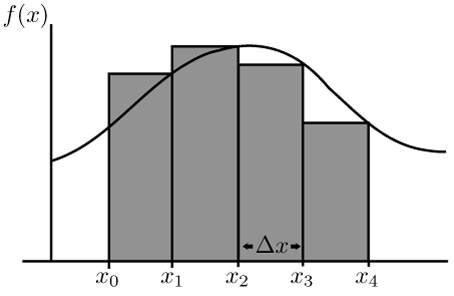
\includegraphics[width=0.5\textwidth]{riemann_1}
      \caption{A function with Right-hand Riemann sum rectangles drawn underneath.}
    \end{figure}

    Riemann sums are not limited to rectangles, however. Another, more accurate method of approximation makes use of trapezoids, whose area formula is comparably simple to that of a rectangle's. Trapezoidal approximation is similar to the result of averaging a left and right approximation. This method makes use of the trapezoid area formula \( A = \frac{1}{2}h(b_1+b_2) \). A Riemann sum constructed with trapezoids takes this form:

    \[ \displaystyle\lim_{n \to \infty}\frac{1}{2}\Delta x\sum_{i=1}^n f(a+i\Delta x) \]

    Historically, Riemann's definition was the first rigourous definition of the integral of a function on an interval. Thus, in Calculus classes today, it is often the first introduction students recieve to the idea of calculating the area under a curve; the AP Calculus Syllabus even specifies Riemann sums as the first material in the Integrals unit.\footnote{http://media.collegeboard.com/digitalServices/pdf/ap/ap-calculus-course-description.pdf}

    As a student who was introduced to integration with Riemann sums, I often wondered: are there other shapes that you could use or approximations similar to Riemann's that would behave similarly? In this paper I intend to investigate just that: are circles a viable shape to use in the fashion of a Riemann sum? How accurate is such an approximation? Does this approximation behave like a Riemann sum in that its limit approaches the real area under the curve?

    In this investigation, I'll derive this approximation (hereafter called the circle sum) in a similar method to how Riemann sums can be derived. I'll then test each of my questions. I'll compare the efficacy of a circle sum versus a similar Riemann sum, as well as examine the behavior of the circle sum as it approaches infinity.

  \section{Derivation}
    The Riemann sum can be simply derived by finding the area of a shape under the curve, summing all such shapes between two bounds, and finally taking the limit of this summation as the number of rectangles approaches infinity. In order to find a circle sum, a similar process will be followed.

    \subsection{Riemann}
      We begin by being given a function \( f(x) \) and a set of bounds \( a \) and \( b \). The width of the workable area is defined as \( b-a \). Thus, we can divide the workable area into \( n \) partitions, each with a width of \( \Delta x = \frac{b-a}{n} \). The right-bound x-value for any such rectangle inside of these bounds can be bound by adding the partition width \( n \) times for the \(n\)th partition. Such a rectangle on the curve has width \( \Delta x \) and height \( f(a+n_i\Delta x) \). Thus, the area of this rectangle is \( f(a+n_i\Delta x)\Delta x \). This rectangle would appear below the function in the manner shown in Figure 2.

      \begin{figure}[h!]
        \centering
        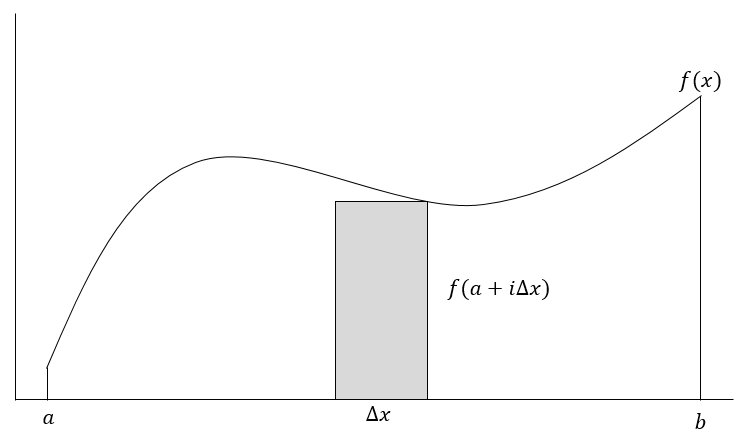
\includegraphics[width=0.8\textwidth]{riemann_deriv_1}
        \caption{A Riemann-style rectangle placed below a curve.}
      \end{figure}

      The sum of the rectangles that exist from \( a \) to \( b \) can be expressed with summation notation:

      \[ A_{total} = f(a+(0)\Delta x)\Delta x + f(a+(1)\Delta x)\Delta x + \dots + f(a+n\Delta x)\Delta x \]

      \[ = \displaystyle\sum_{i=0}^n f(a+i\Delta x)\Delta x \]

      \( A_{total} \) is represented by the shaded green areas in Figure 3.

      \begin{figure}[h]
        \centering
        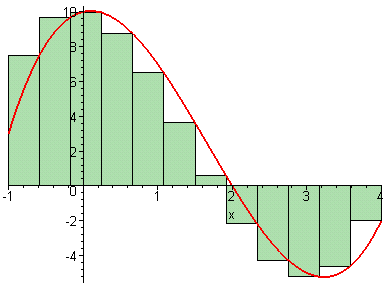
\includegraphics[width=0.5\textwidth]{riemann_2}
        \caption{A function with Riemann rectangles placed underneath it.}
      \end{figure}

      When we take the limit of \( A_{total} \) as the number of partitions, \( n \), approaches infinity, we find that \( A_{total} \) approaches \( A_{real} \), given by integrating the function from \( a \) to \( b \).

      \[ \displaystyle\lim_{n \to \infty}\sum_{i=0}^n f(a+i\Delta x)\Delta x = \int\limits_a^b f(x)dx \]

    \subsection{Circle}
      There are two concievable methods for using circles to determine the area underneath a function. The first stacks circles with diameter \( \Delta x \) up to the curve, and sums their areas. This is shown in Figure 4. The second finds the largest possible circle which is tangential to the curve at a given \( x \) and sums the areas of the circles that do not overlap and which fit inside the bounds. This is shown in Figure 5.

      \begin{figure}[h]
        \centering
        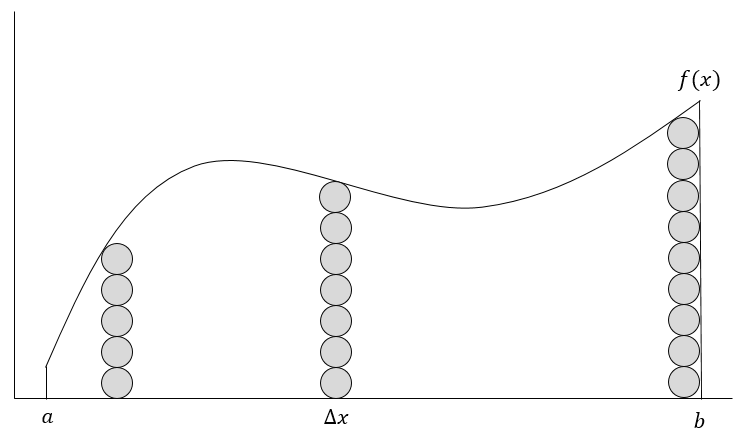
\includegraphics[width=0.8\textwidth]{circle_example_1}
        \caption{A stacked-circle style approximation.}
      \end{figure}

      \begin{figure}[h]
        \centering
        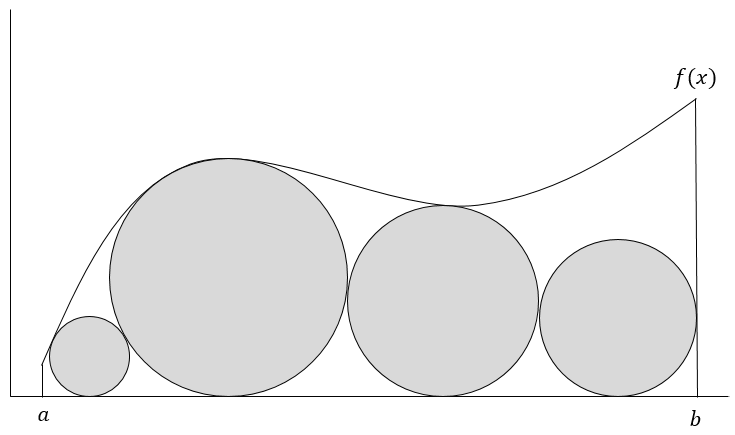
\includegraphics[width=0.8\textwidth]{circle_example_2}
        \caption{A filled-circle style approximation.}
      \end{figure}

      \subsubsection{Filled Circles}
        Figure 5 somewhat gives away the failings of the Filled Circle method. Because circles cannot overlap, they cannot appropriatley grow to fit the area underneath the curve. This means that the approximation will have huge failings when it comes to estimating the real area underneath the curve. In order to examine this method as we would a Riemann sum, by examining a variable which approaches infinity, we would need to continue to add circles into the empty space, a process which is beyond the scope of this invesitgation. Finding the optimal number of circles that will fit under the curve is a problem of \emph{circle packing}, which examines how to fit circles into an enclosed space.

      \subsubsection{Stacked Circles}
        This method is the most likely to behave like a Riemann sum because it creates smaller and smaller shapes to fit under the curve. However it might suffer in accuracy due to \emph{circle packing}, which immediatley introduces a problem with computing a Riemann-style circle sum: a circle has approximatley 78\% the area of an similarly-sized square (see Figure 6). It is to be discovered if this discrepancy will disappear as the number of circles increases to infinity.

        \begin{figure}[h]
          \centering
          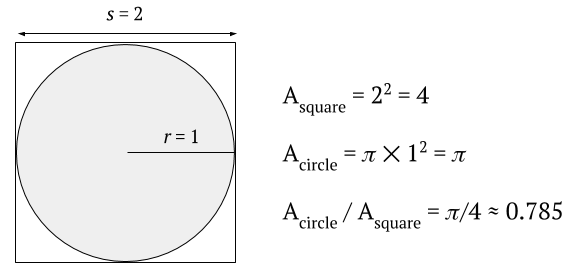
\includegraphics[width=0.8\textwidth]{circle_packing}
          \caption{A circle is circumscribed within a square. The circle has 78\% of the area of the square.}
        \end{figure}

        We can begin with the same set of givens for a Riemann sum: a function, \( f(x) \), and a set of bounds, \( a \) and \( b \). This workable area, with \( n \) partitions, has a partition width of \( \Delta x = \frac{b-a}{n} \). Each circle will have diameter \( \Delta x \). Therefore each will have radius \( r = \frac{\Delta x}{2} \) and area \( \pi \left(\frac{\Delta x}{2}\right)^2 \). We can find the number of circles required for a given \( x \) by dividing the function value by the diameter of a circle. Therefore, for a given \( x \) in partition \( n \), the area of the circles beneath it is:

        \[ A_{stack} = \frac{f(a+n_i\Delta x)}{\Delta x} \times \frac{\pi \Delta x^2}{4} \]

        \[ = \frac{f(a+n_i\Delta x)\pi\Delta x}{4} \]

        Substituting \( \Delta x = \frac{b-a}{n} \) back in, this simplifies to

        \[ A_{stack} = \frac{f(a+n_i(\frac{b-a}{n}))(b-a)\pi}{4n} \]

        Therefore, the sum of these circles over a function from \( a \) to \( b \) partitioned \( n \) times can be expressed in summation notation as

        \[ A_{total} = \displaystyle \sum_{i=0}^n \frac{f(a+i(\frac{b-a}{n}))(b-a)\pi}{4n} \]

  \section{Accuracy}
    Now that we have a general equation for the circle sum, we can test it. Let \( f(x) = x^2 + 1; [a,b] = [0,1]; n = 10 \). A circle sum appears thusly:

    \[ A_{total} = \displaystyle \sum_{i=0}^{10} \frac{f(\frac{i}{10})\pi}{40} = \frac{\pi}{40} + \frac{1.01\pi}{40} + \dots + \frac{2\pi}{40} = \frac{297}{800}\pi \approx 1.166 \]

    Comparatively, a rectangular right-hand Riemann sum for these givens produces the following output:

    \[ A_{total} = \displaystyle \sum_{i=0}^{10} \frac{f(\frac{i}{10})}{10} = \frac{1}{10} + \frac{1.01}{10} + \dots + \frac{2}{10} = 1.485 \]

    Interestingly, the effects of circle packing are already visible. The approximate area acquired through the circle sum is 78\% of the area acquired through the rectangular sum.

    \[ \frac{1.166}{1.485} \approx 0.7851 \]

    One characteristic of right-hand Riemann sums is that they tend to underestimate while handling concave curves, and overestimate while handling convex curves. This error is visible in Figure 3: when the curve is convex (\([-1,0],[2,3] \)), the rectangles are slightly too large; when the curve is concave, they are slighly too small. It is possible that our circle sum would exhibit the same tendency. Let's test the circle sum again, this time modifying our \( f(x) \) to be concave.

    \[ f(x) = -x^2 + 1 \]

    \[ A_{total} = \displaystyle \sum_{i=0}^{10} \frac{f(\frac{i}{10})\pi}{40} = \frac{\pi}{40} + \frac{0.99\pi}{40} + \dots + \frac{0\pi}{40} = \frac{143\pi}{800} \approx 0.562 \]

    \[\displaystyle \int\limits_0^1 (-x^2+1)dx = \frac{2}{3} \approx 0.66667 \]

    It would appear that the circle sum underestimates, no matter the shape of the curve. This makes sense, because of the lost space created by circle packing. However, we now must examine the circle sum's behavior at infinity, to discover if infinitley small circles will perfectly pack to equal the integral of the function.

  \section{Sums at Infinity}
    Riemann sums converge to the real value of the integral when we let the number of partitions go to infinity. This is expressed as

    \[ \displaystyle\lim_{n \to \infty}\sum_{i=1}^{n} f(x^*_i) \Delta x = \int\limits_a^b f(x)dx \]

    This property can be confirmed by finding a closed-form version of a Riemann sum, where \( n \) is left undefined. We then examine that form by taking the limit as \( n \) goes to infinity. The result is the real value of the integral over those bounds. For a circle sum, the same process will be followed.

    \subsection{Riemann}
      In order to find the closed form of a Riemann sum we must leave \( n \) undefined. For this example, we will use the same givens as used in Section 2.2.2: \( f(x) = x^2 + 1 \) on \( [a,b] = [0,1] \). Therefore \( \Delta x = \frac{1}{n} \).

      \[ A_{total} = \displaystyle\sum_{i=0}^n f(\frac{1}{n}i)\times\frac{1}{n} = \sum_{i=0}^n \frac{f(\frac{i}{n})}{n} = \frac{(\frac{0}{n})^2+1}{n} + \frac{(\frac{1}{n})^2+1}{n} + \dots + \frac{(\frac{n}{n})^2+1}{n} \]
      \[ = \frac{1}{n}\left[ \left( \left(\frac{0}{n}\right)^2 + 1 \right) + \left( \left(\frac{1}{n}\right)^2 + 1 \right) + \dots + \left( \left(\frac{n}{n}\right)^2 + 1 \right) \right] \]
      \[ = \frac{1}{n}\left[ \left( \frac{0}{n} \right)^2 + \left( \frac{1}{n} \right)^2 + \dots + \left( \frac{n}{n} \right)^2 \right] + \frac{n}{n} \]
      \[ = \frac{1}{n^3}\left[ \frac{n(n+1)(2n+1)}{6} \right] + 1 = \frac{(n+1)(2n+1) + 6n^2}{6n^2} \]
      \[ = \frac{8n^2+3n+1}{6n^2} = \frac{4}{3} + \frac{1}{3n} + \frac{1}{6n^2} \]
      \[ \displaystyle\lim_{n \to \infty}\left(\frac{4}{3} + \frac{1}{3n} + \frac{1}{6n^2} \right) = \frac{4}{3} = \int\limits_0^1 (x^2+1)dx \]

    \subsection{Circle}
      Now let's do the same thing for a circle sum. \( f(x) = x^2 + 1, [a,b] = [0,1]\).

      \[ A_{total} = \displaystyle\sum_{i=0}^n \frac{f(\frac{i}{n})\pi}{4n} = \frac{\left((\frac{0}{n})^2+1\right)\pi}{4n} + \frac{\left((\frac{1}{n})^2+1\right)\pi}{4n} + \dots + \frac{\left((\frac{n}{n})^2+1\right)\pi}{4n} \]
      \[ = \frac{\pi}{4n}\left[ \left( \left(\frac{0}{n}\right)^2 + 1 \right) + \left( \left(\frac{1}{n}\right)^2 + 1 \right) + \dots + \left( \left(\frac{n}{n}\right)^2 + 1 \right) \right] \]
      \[ = \frac{\pi}{4n}\left[ \left( \frac{0}{n} \right)^2 + \left( \frac{1}{n} \right)^2 + \dots + \left( \frac{n}{n} \right)^2 \right] + \frac{n}{n} \]
      \[ = \frac{\pi}{4n^3}\left[ \frac{n(n+1)(2n+1)}{6} \right] + 1 = \frac{\pi(n+1)(2n+1) + 24n^2}{24n^2} \]
      \[ = \frac{26\pi n^2+3\pi n+\pi}{24n^2} = \frac{26\pi}{24} + \frac{3\pi}{24n} + \frac{\pi}{24n^2} \]
      \[ \displaystyle \lim_{n \to \infty}\left(\frac{26\pi}{24} + \frac{3\pi}{24n} + \frac{\pi}{24n^2}\right) = \frac{26\pi}{24} \approx 3.403 \]

      It would appear that the circle sum has severely \emph{overapproximated} the real area underneath the curve.


\end{document}
